%!TEX root = paper.tex
%%%%%%%%%%%%%%%%%%%%%%%%%%%%%%%%%%%%%%%%%%%%%%%%%%%%%%%%%%%%%%%%%%%%%%%%%%%%%%%%
\section{Characterizing Platforms and Games}
\label{sec:background}

This section covers the basic characteristics of different gaming platform types, most notably the traditional  \textit{à la carte} model and \textit{fixed fee subscription} cloud gaming approaches. Section~\ref{sec:engagement} will then use these characteristics to reason about player engagement and budget considerations.

%%%%%%%%%%%%%%%%%%%%%%%%%%%%%%%%%%%%%%%%%%%%%%%%%%%%%%%%%%%%%%%%%%%%%%%%%%%%%%%%
\subsection{Platform Characteristics}\label{subsec:platform-characteristics}

Below, currently active (cloud and other) gaming platforms are examined with regards to pricing models and hardware requirements and costs. The information presented was collected between July 2015 and February 2016. All costs are from an European, specifically German, perspective. If a product is not available in this region, the prices are converted using the most recent currency exchange rates.

\subsubsection{Video Game Consoles}

A classical approach to video gaming is using dedicated consoles with physical copies of game media (e.g., a Blue-ray Disc) bought at a retailer. The price for (non-portable) consoles varies but usually lies between \SI{300}[\EUR]{} and \SI{400}[\EUR]{} for the latest console generation, i.e., \textit{Wii U}, \textit{PlayStation 4}, and \textit{Xbox One}. New, major game releases are mostly priced at either \SI{60}[\EUR]{} or \SI{70}[\EUR]{}. Once on the market, the game prices decrease rather slowly. In recent years, retail stores have been complemented with console-specific, proprietary digital distribution services that also offer the latest game at the full price. These official stores are usually exclusive vendors for digital game codes where competitors are excluded.
Subscription fees often apply for the multiplayer mode of games, e.g., \textit{PlayStation Plus} or \textit{Xbox Live Gold} with annual prices of \SI{50}[\EUR]{} and \SI{60}[\EUR]{}, respectively. These services also include access to a small, monthly changing palette of older titles.


\subsubsection{The PC Gaming Ecosystem}
\label{sec:pcgaming}

The rise of easy-to-use digital distribution platforms and the independent (``indie'') game scene reinvigorated PC gaming just a few years ago. Today, PC gaming is dominated by large digital marketplaces, with \steam being the largest. The platform has about $10$ million concurrent users at most times of the day. It periodically offers large, often seasonal, sales of recent games at greatly reduced prices (rebates of 75\% for a year-old game are not uncommon). In addition, many resellers offer digital codes for other platforms, often at much lower prices.
Major releases on PC are usually priced between \SI{50}[\EUR]{} and \SI{60}[\EUR]{}. However, due to the competition between the vendors, the digital retail prices are significantly lower even at launch, and also drop more quickly. Another recent trend are game bundles, which especially prevalent in the indie games scene, commonly offered with a pay-what-you-want model. \textit{Humble Bundle}\footnote{\url{https://www.humblebundle.com/}} is a prominent example. 

Hardware viable for PC gaming starts at about \SI{500}[\EUR]{} but has practically no upper limit for enthusiasts (especially the \gls{GPU} is a cost driver, yet essential for modern PC gaming). Thus, the barrier for customers to start PC gaming is higher than for consoles, which is, however, compensated by an increased flexibility and longevity of hardware.


\subsubsection{Geforce NOW}

NVIDIA's cloud gaming service %\footnote{\url{https://shield.nvidia.com/games/geforce-now}}
is available in North America and select European countries. Like in all cloud gaming services  games are executed and rendered ``in the cloud'' (i.e., in remote data centers), and an audio/video stream is sent back to the player. In Germany the service currently offers $68$ PC titles for a monthly subscription fee of \SI{10}[\EUR]{}. An additional per-game one-time fee between \SI{13}[\EUR]{} and \SI{60}[\EUR]{} is charged for the access to the $19$ most prominent and recent games. The service is delivered from six specialized data center locations (Dublin and Frankfurt in Europe).

The requirements to use this service are rather steep, demanding \SI{50}{\mega\bit\per\second} for a full 1080p60\footnote{\label{foot:rate}Please note: This frame rate of \SI{60}{\hertz} represents the rate of the video encoder and not the game's actual frame rate, which might be considerably lower depending on the complexity of the game.} stream (\SI{10}{\mega\bit\per\second} in order to use the service at all) and a maximum \acrshort{RTT} of \SI{60}{\milli\second} to one of the data centers. In addition, streaming is exclusive to \textit{SHIELD} devices which start at \SI{200}[\EUR]{}.

\subsubsection{PlayStation Now}

Sony's cloud gaming service offers to stream titles from previous PlayStation generations, as the latest console generation lacks backwards compatibility. It is currently available in North America and the UK, with a closed beta running in other European countries and Japan. The offered titles and exact pricing vary from country to country. For the UK, about $190$ titles are available, and most titles are covered by the monthly subscription fee of about \SI{17}[\EUR]{}. All titles are also available through a separate rental service, costing about \SI{4}[\EUR]{} for \SI{48}{\hour} and \SI{10}[\EUR]{} for one month of access. This is in addition for the device cost, as the service is only available on PlayStation 4 and 3 consoles as well as some select Sony TVs and other devices with extra game controller.

The streaming itself is performed at a resolution of 720p60 requiring a \SI{5}{\mega\bit\per\second} connection. Reports on the video quality have been rather mixed.\footnote{\url{http://www.eurogamer.net/articles/digitalfoundry-2015-hands-on-with-playstation-now}}



%%%%%%%%%%%%%%%%%%%%%%%%%%%%%%%%%%%%%%%%%%%%%%%%%%%%%%%%%%%%%%%%%%%%%%%%%%%%%%%%
\subsection{Characteristics of Games}

Following the discussion of gaming platform characteristics, the attention now turns to the properties of the actual games offered on the various platforms: number of games, ages, lengths, prices, and review scores. Table~\ref{tab:game-stats} provides an overview of the data.
In order to investigate these characteristics, data was collected from multiple sources and merged (with a few instances of omission and double-count) into a data base. In the interest of repeatability and reproducibility, all of the data reported on in this work, as well as the code used to collect and process it, can be found in public repositories\footnote{The main repository can be found at \url{https://github.com/mas-ude/cost-of-cloud-gaming}}. Please note that due to space constraints and the multidimensional nature of the dataset, only a limited number of findings can be  presented in this paper.

%%%%%%%%%%%%

\begin{table*}
\centering
\caption{Game characteristics on the investigated platforms. Title counts from Web/API scraping, lengths from \hltb, ages and review scores from \metacritic.}
\label{tab:game-stats}
	\begin{tabu}{X[2]|X[r]X[r]X[r]X[r]X[r]X[r]X[r]}
	\toprule
	Service & Titles & Age $\mu$ & Age $\sigma$ & Length $\mu$ & Length $\sigma$ & Score $\mu$ & Score $\sigma$ \\
	\midrule
	\gfnow & $68$ & \SI{2.87}{\year} & \SI{1.95}{\year} & \SI{14.65}{\hour} & \SI{14.44}{\hour} & $75.9$ & $9.44$ \\
	\psnow & $191$ & \SI{5.24}{\year} & \SI{2.55}{\year} & \SI{12.26}{\hour} & \SI{15.47}{\hour} & $76.72$ & $11.43$ \\
	\steam & $7749$ & \SI{3.36}{\year} & \SI{3.95}{\year} & \SI{13.02}{\hour} & \SI{20.49}{\hour} & $71$ & $12$ \\
	\bottomrule
	\end{tabu}
\end{table*}


%%%%%%%%%%%%
\subsubsection{Number of Games}

This basic metric quantifies the range of games on offer. The two cloud platforms offer a very limited number of games when compared to the games available on \steam, which itself again only represents a subset of all games available either on the PC platform (\metacritic lists $16192$) or across all platforms ($45803$ listed on the site). Two possible, simple explanations for the low game count on the cloud platforms come to mind: One is that they were launched relatively recently (2015) in comparison to \steam (2003), leaving little time for the range of games to grow. Secondly, the choice of games for a cloud gaming platform is necessarily curated by the platform operator due to compatibility and performance reasons. This usability burden shifts to the end user for digital storefronts like \steam, allowing these platforms to offer a larger variety of games, including ones that are very demanding on the hardware.


%%%%%%%%%%%%
\subsubsection{Game Ages}

The age of a game is computable from its release date. To this end, the \metacritic\footnote{\url{http://www.metacritic.com/}} page which aggregates reviews of video games (and other media) was scraped\footnote{\url{https://github.com/mas-ude/metacritic_scraper}}. Game ages appear to be relatively high for all of the investigated platforms, and particularly so for \psnow. It might be considered a special case, as it is specifically advertised as a backwards compatibility for older, pre-PlayStation 4 games that do not run on the latest Sony platform any more. For \steam, the distribution is significantly skewed towards recent titles: A quarter of games are less than $10$ months old, and the median is at $21$ months. The distribution's tail extends well beyond $25$ years (due to re-releases of ``classic'' games on the platform).


%%%%%%%%%%%%
\subsubsection{Game Lengths}

Game publishers are usually not outspoken about the intended playthrough length of games, nor do all games necessarily have a logical end, and thus a useful definition of a playthrough length. However, players may self-report their experienced playthrough times on sites like \hltb\footnote{\url{http://howlongtobeat.com/}}, on whose data this analysis is based\footnote{\url{https://github.com/mas-ude/gamelengths-scraper}}.
Figure~\ref{fig:gamelengths-violin} shows the distribution of aggregated game lengths for the three platforms under investigation, and an ``overall'' distribution that includes further platforms and gaming systems. Among the three platforms, the mean and median reported game lengths (approximately \SI{14}{\hour}) are largest for \gfnow. In contrast to the curated choice of games on the Cloud systems, \steam also offers shorter and longer games.


\begin{figure}[!t]
	\centering
	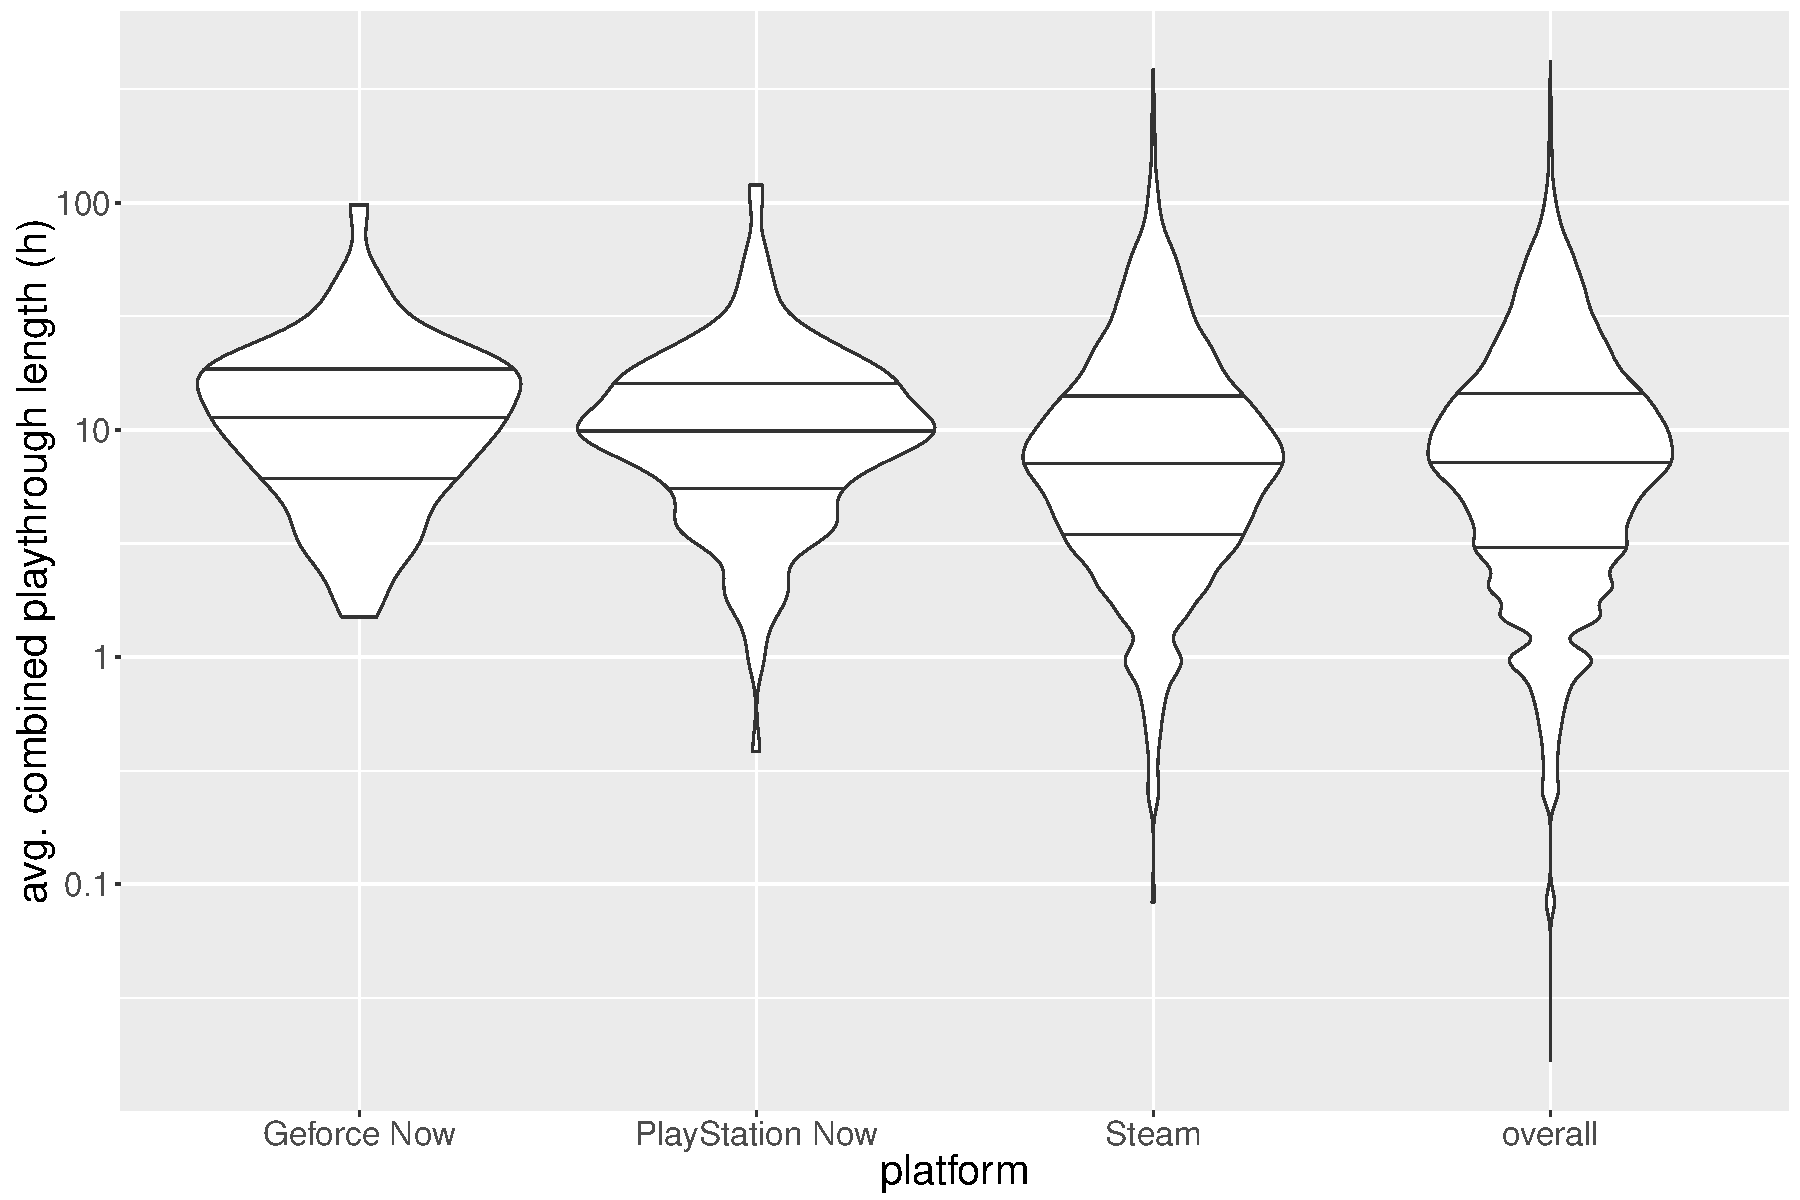
\includegraphics[width=1.0\columnwidth]{images/gamelengths-by-platform-violin.pdf}
	\caption{Violin plot of the per-platform average game lengths from \hltb. The number of games per bin are $68$, $209$, $7764$, and $18433$; quartiles indicated by horizontal lines.}
\label{fig:gamelengths-violin}
\end{figure}



%%%%%%%%%%%%
\subsubsection{Game Prices}

Trying to compare the prices per game is a difficult endeavor, due to the mixed approach of both cloud gaming platforms. The \gfnow subscription gives access to a subset of its catalog that can be extended by purchasing additional games. Similarly, \psnow has a base subscription catalog and additional, rent-able titles. But in addition, every title can also be rented without the need for an active subscription.
Nevertheless, for \steam it is possible to discuss unit prices: Using the official \acrshort{REST} \acrshort{API}, name and current price of each game were fetched at three different points in time\footnote{\url{https://github.com/mas-ude/steam-data-stats}}. This data was combined with \acrshort{API} data from the 3rd-party site \textit{SteamSpy}\footnote{\url{https://steamspy.com}}, which parses all publicly visible \steam user profiles. Subsequently, \textit{SteamSpy} estimates statistics on the size of the player base and the time each player spends with a title. Furthermore, the site provides a heuristic projection of the total number of owners of each listed title on \steam. Using the combined data, additional perspectives can be given.

\begin{table}
\centering
\caption{Average prices for \steam games.}
\label{tab:steam-price-stats}
\begin{tabu}{X[2]|X[r]X[r]X[r]}
	\toprule
	& \textbf{2015-07-14} & \textbf{2015-10-30} & \textbf{2016-02-06} \\
	\midrule
	\textbf{Portfolio price (€)} & $10.11$ & $8.47$ & $5.65$ \\
	\textbf{Weighted price (€)} & $12.39$ & $10.21$ & $5.30$ \\
	\bottomrule
\end{tabu}
\end{table}

Table~\ref{tab:steam-price-stats} shows the development of average \steam game prices for the three measurements taken. Two different types of averages are shown: The portfolio price which averages over all current game prices, and the weighted price which is the product of game price and estimated number of owners, averaged over the total number of games owned. Strong temporal effects are evident from either metric. Note that the last measurement shortly predates 2016's Lunar New Year, around which \steam ran a large seasonal sales campaign\footnote{\url{https://store.steampowered.com/oldnews/20313}}.

\begin{figure}[!t]
	\centering
	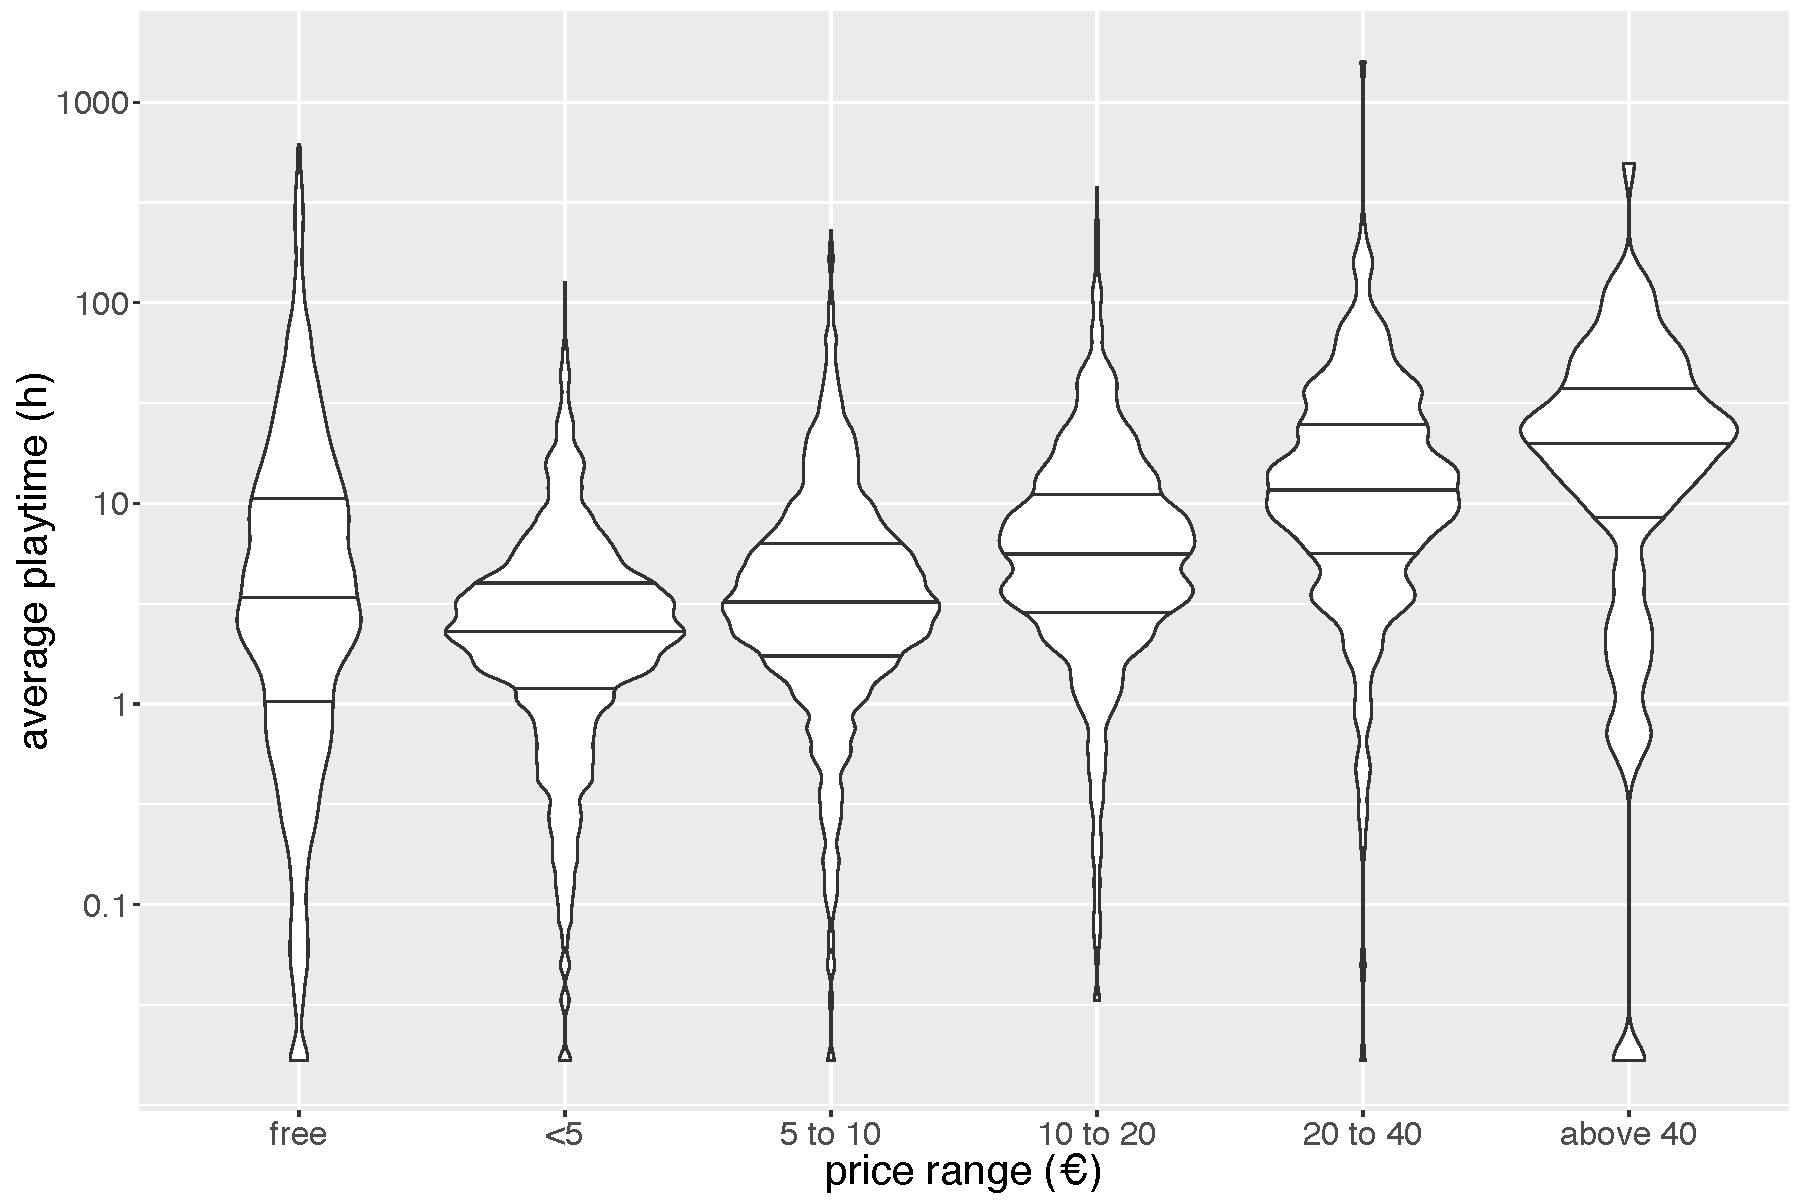
\includegraphics[width=1.0\columnwidth]{images/steam-cost-vs-playtime-non-sale.pdf}
	\caption{Violin plot of the average playtime of \steam games, broadly categorized by their prices. The number of games per bin are $1122$, $2177$, $1946$, $1106$, $328$, and $90$.}
\label{fig:steam-cost-vs-playtime-violin}
\end{figure}

Figure~\ref{fig:steam-cost-vs-playtime-violin} breaks down the distribution of average playtimes per game price range. The game price ranges are chosen so as to roughly separate the prevalent modes of the price distribution.
Playtime is defined as the time game owners spend playing a game, as recorded by the \steam platform and scraped from \textit{SteamSpy}. As can be seen, the playtimes generally increase with the price range; unfortunately, the data does not explain the cause: E.g., more expensive games might have more playable content, causing the playtime to increase. Conversely, higher upfront costs may incite players to spend more time regardless of game quality, thus avoiding regret for the expense. On the far left in the Figure, playtimes of ``free'' titles (including free-to-play games with monetization options other than an upfront payment) span almost the whole playtime range with less pronounced prevalences.
Due to the strong popularity of \steam in PC gaming (even physical retail copies often require using the online service nowadays) this set also gives a good general overview of the dimensions of PC gaming in general.


%%%%%%%%%%%%
\subsubsection{Review Scores}

The final characteristic in this analysis are game review scores as given by professional gaming media outlets. This relies on the \metacritic dataset again. This set covers review scores for all current and historic gaming platforms. The review scores are aggregated to average scores ranging between $0$ and $100$. Some \metacritic-internal weighing factors are applied to express the importance of some media outlets over others.
The average scores seem quite similar across all services, albeit with a slightly lower $\sigma$ for \gfnow. Figure~\ref{fig:scores-by-platform} shows the distribution of review scores per platform. Both Cloud services seem to favor certain score levels. Specifically, their lowest quartiles (representing the worst-rated games on these platforms) reach much higher values than \steam's. This could be an effect of the Cloud systems curating the game offer to focus on highly-rated (and thus perhaps more attractive) titles. \steam on the other side is a more or less open platform, where every game publisher can sell their games at their own volition (platform operator collects a commission fee for sales). Consequently, it is reasonable to assume more variation in the quality of games, which could in turn lead to mixed reviews.

\begin{figure}[!t]
	\centering
	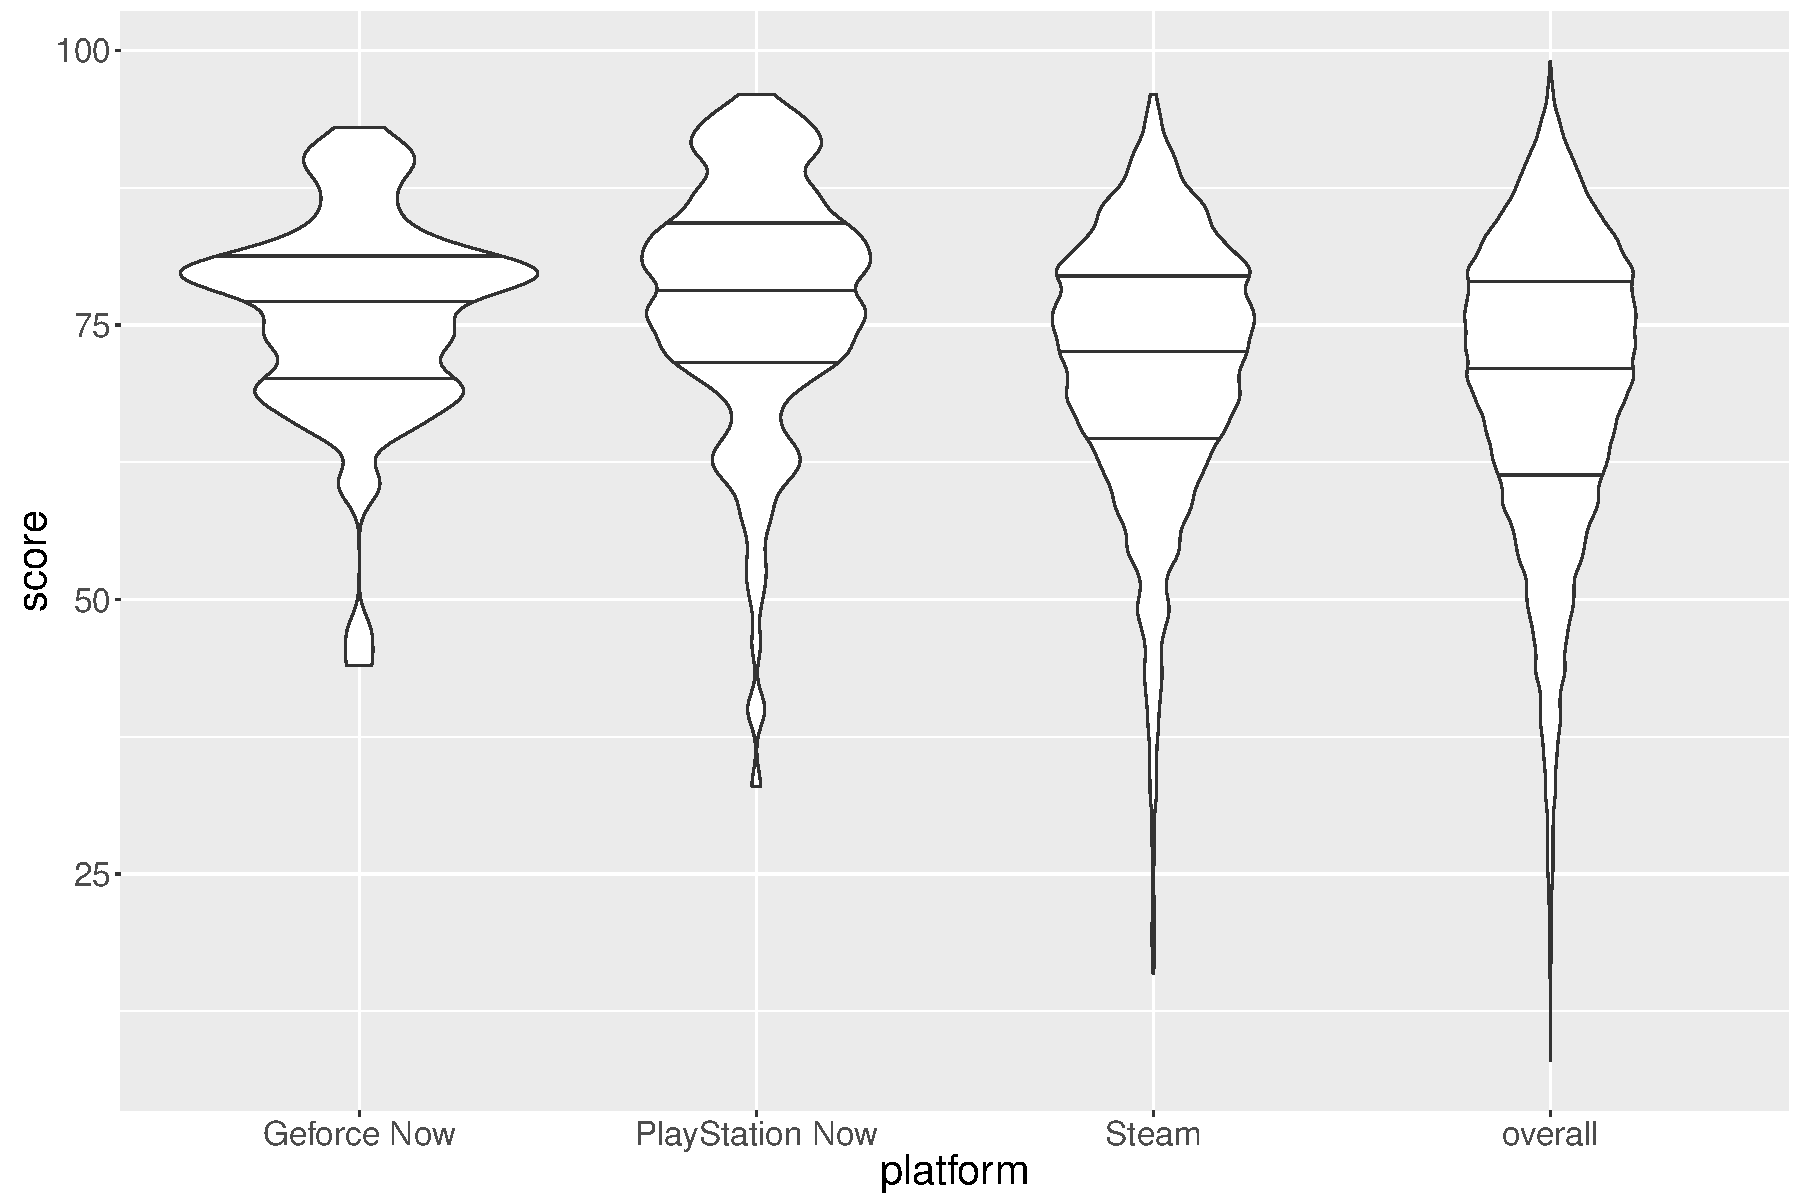
\includegraphics[width=1.0\columnwidth]{images/scores-by-platform-violin.pdf}
	\caption{Violin plot of aggregated review scores per platform. The number of games per bin are $68$, $209$, $7759$, and $46197$. Overall represents all games scraped from \metacritic.}
\label{fig:scores-by-platform}
\end{figure}

